\section{Introduction}
\label{sec:introduction}
The main goal of this work is to analyze a circuit using 3 methods: mesh
(Section ~\ref{sec:mesh analysis}) and nodal (Section ~\ref{sec:nodal analysis}) analysis and using an \textit{ngspice} simulation (Section ~\ref{sec:simulation}).\footnote{To get the values of resistance for each resistor and other data, we used the number 96514 (the lowest of the three student Id's).}\\

Our circuit (Figure ~\ref{fig:circuit}) consists of 7 resistors, 2 voltage sources - 1 independent, and 1 current controlled dependent one, and 2 current sources - 1 independent, and 1 voltage controlled dependent one. There are 4 meshes and 8 nodes. Voltage source $V_a$ is in series with resistor 1; Resistor 2 and current source $I_b$, and resistors 6 and 7 ares also connected in series. \\
\begin{figure}[H] \centering
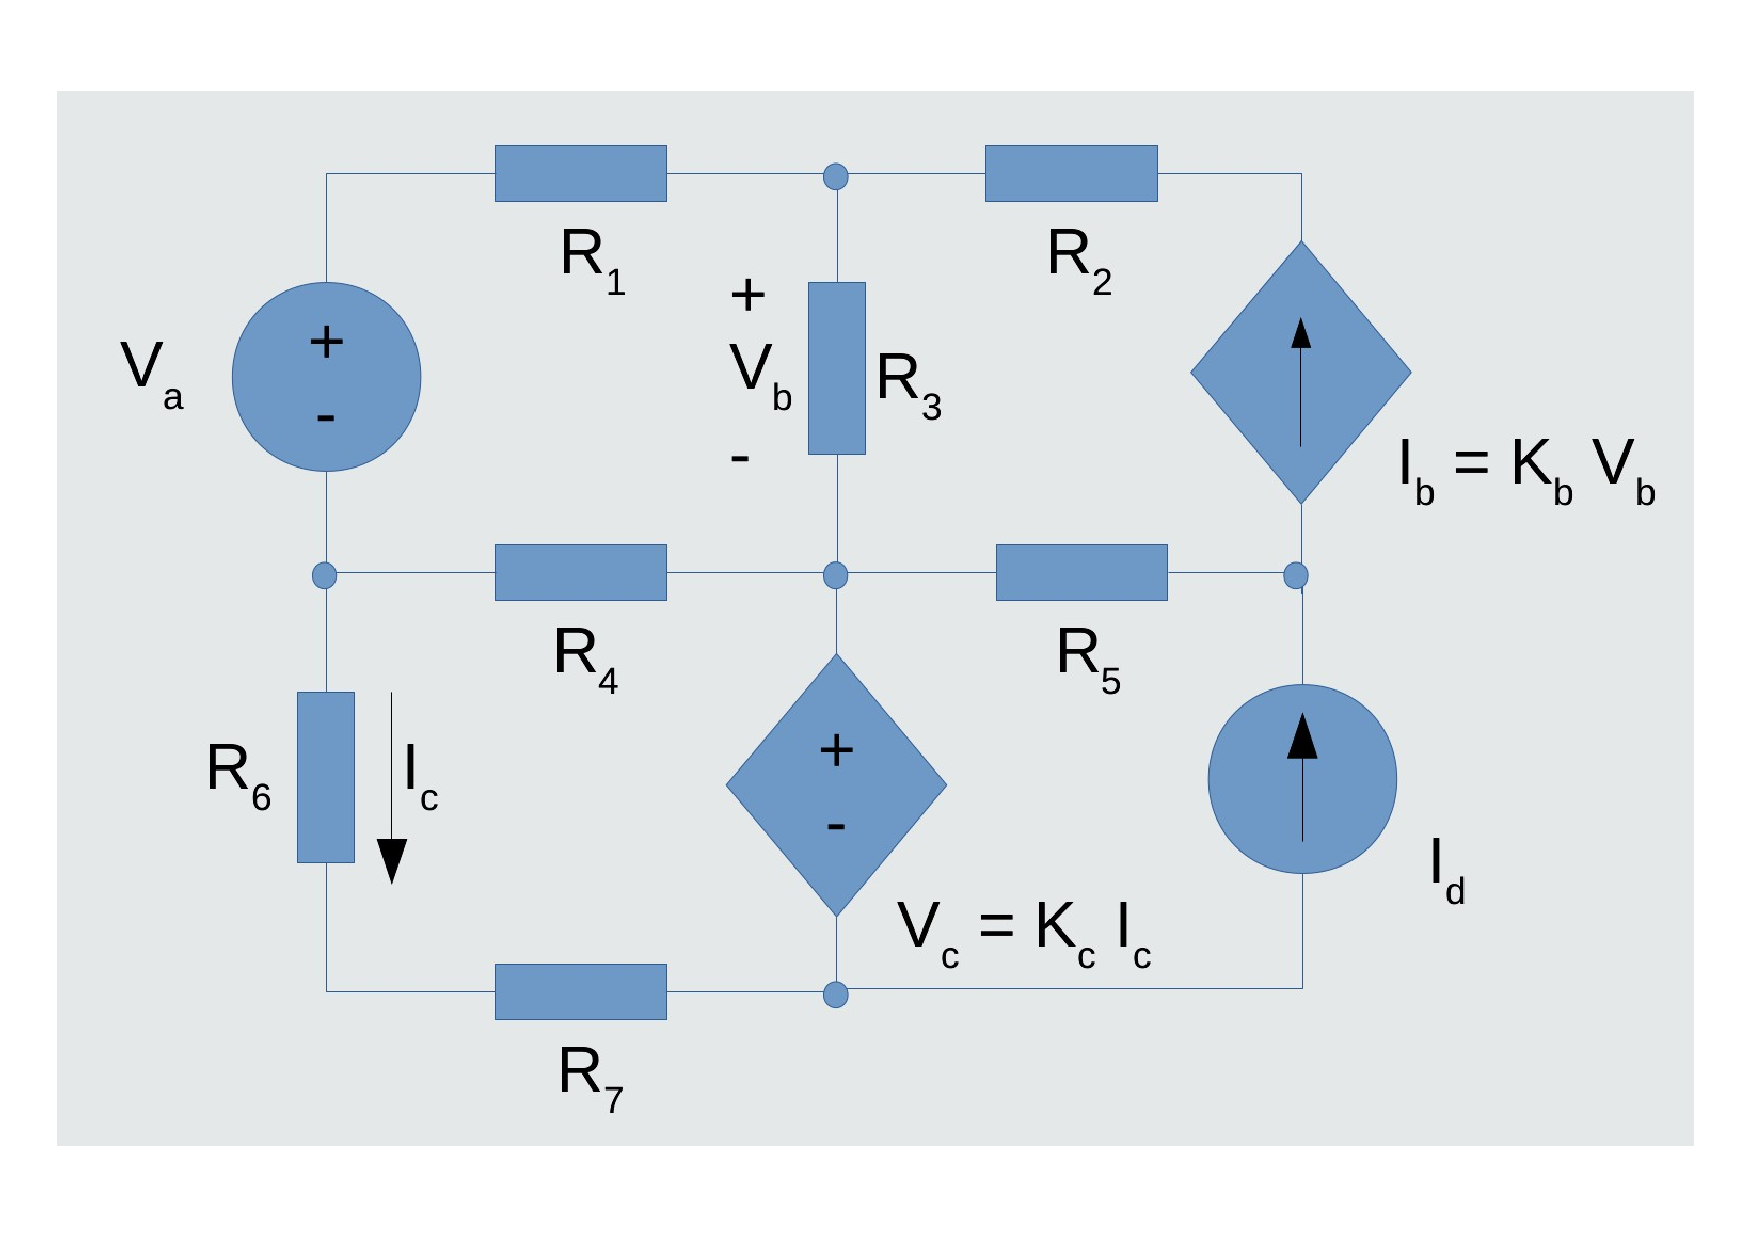
\includegraphics[width=0.8\linewidth]{circuit.pdf}
\caption{Circuit}
\label{fig:circuit}
\end{figure} 
We wrote a system of equations for each theoretical method (mesh and nodal), from Kirchhoff and Ohm's Laws. To get the solutions for these analysis, we used \textit{octave}, which solved our systems of equations efficiently and gave us all currents and voltages for each resistor. We then used \textit{ngspice} to get a simulation of this circuit, expecting to obtain the same results in all three methods. We compared the results from different methods in the conclusion (Section ~\ref{sec:conclusion}).\\
